\documentclass[12pt,a4paper]{article}
\usepackage[utf8]{inputenc} %polskie znaki
\usepackage[T1]{fontenc}	%polskie znaki
\usepackage{amsmath}		%matematyczne znaczki :3
\usepackage{enumerate}		%Dodatkowe opcje do funkcji enumerate
\usepackage{geometry} 		%Ustawianie marginesow
\usepackage{graphicx}		%Grafika
\usepackage{wrapfig}		%Grafika obok textu
\usepackage{float}			%Allows H in fugire
\usepackage{hyperref}		%Allows hyperlinks
%\pagestyle{empty} 			%usuwa nr strony
\usepackage{todonotes}		%Todo notatki
\usepackage{lipsum}         %Lorem text
\usepackage{ntheorem}   	% for theorem-like environments
\usepackage{mdframed}   	% for framing
\usepackage{subcaption}		% subfigure (image placing)
\usepackage{pdfcomment}		% Komentarze (z bazowego pdf'a)
\usepackage{xparse}			% New commands with optional arguments
\usepackage{ifthen}			% If then - funkcje!
\usepackage{expl3}			% Deklarowanie zmiennych
\usepackage{pgf}			% Aktualne rachunki \pgfmathparse{}

\newgeometry{tmargin=2cm, bmargin=2cm, lmargin=2cm, rmargin=2cm} 

%Counter commands{
	\newcounter{counter} % Creates a new counter
	\setcounter{counter}{1} % Sets the counter to 5
	\newcommand{\counter}[1]{
		\arabic{#1} \stepcounter{#1} 
	}
	\newcommand{\counterreset}[1]{\setcounter{#1}{1}}
	%}

%Define styles{
	\theoremstyle{break}
	\theoreminframepreskip{0.5cm}
	\theoremheaderfont{\bfseries}
	\newmdtheoremenv[%
	linecolor=white,%
	innertopmargin=\topskip,
	shadowsize=0,%
	innertopmargin=5,%
	innerbottommargin=5,%
	leftmargin=10,%
	rightmargin=10,%
	backgroundcolor=gray!20,%
	innertopmargin=0pt,%
	ntheorem]{zad}{Zadanie}
	
	\mdfdefinestyle{zadanie}{
		linecolor=white,%
		innertopmargin=5,%
		innerbottommargin=5,%
		leftmargin=10,%
		rightmargin=10,%
		backgroundcolor=gray!20,%
		innertopmargin=8,
		innerbottommargin=8,
		skipabove = 5,
	}
	\mdfdefinestyle{wzor}{
		linecolor=cyan,%
		linewidth=2pt,%
		innertopmargin=8,
		innerbottommargin=8,
		leftmargin=10,%
		rightmargin=10,%
		backgroundcolor = white, 
		fontcolor = black,
		skipabove = 5,
		skipbelow = 5,
	}
	%}

%Zadania templatex%{
	\newcommand{\Wzor}[1]{
		\begin{mdframed}[style=wzor]
			\centering #1
		\end{mdframed}
	}
	\newcommand{\ZadanieTextowe}[1]{
		\begin{mdframed}[style=zadanie]
			\textbf{Zadanie \counter{counter} } \\
			#1
		\end{mdframed}
	}
	\newcommand{\Zadanie}[2]{
		\ZadanieTextowe{#1}
		#2
	}
	\newcommand{\ZadanieABCD}[6]{
		\ZadanieTextowe{#1}
		#2 \\\\
		\begin{tabular}{p{7cm} p{7cm}}
			\textbf{A. }#3&
			\textbf{B. }#4\\\\
			\textbf{C. }#5&
			\textbf{D. }#6\\
		\end{tabular}
	}
	\newcommand{\ZadanieABCDEF}[8]{
		\ZadanieTextowe{#1}
		#2 \\\\
		\begin{tabular}{p{7cm} p{7cm}}
			\textbf{A. }#3&
			\textbf{B. }#4\\\\
			\textbf{C. }#5&
			\textbf{D. }#6\\\\
			\textbf{E. }#7&
			\textbf{F. }#8\\\\
		\end{tabular}
	}
	
	\newcommand{\ZadaniePF}[3]{
		\ZadanieTextowe{#1}
		\textbf{Wybierz odpowiedź prawda (P) lub fałsz (F).} \\\\
		\PF{#2}{#3}
	}
	\newcommand{\PF}[2]{\setlength\arrayrulewidth{2pt}{
		\def\arraystretch{2}
		\begin{tabular}{|p{14cm}| c|c|}\hline
			#1 & {\Large P} & {\Large F}\\\hline
			#2 & {\Large P} & {\Large F}\\\hline
		\end{tabular}}
	}
	\newcommand{\PFEmpty}[2]{\setlength\arrayrulewidth{2pt}{
			\def\arraystretch{2}
			\begin{tabular}{|p{14cm}| c|}\hline
				#1 & {\Large $\dots$}\\\hline
				#2 & {\Large $\dots$}\\\hline
		\end{tabular}}
	}
	\newcommand{\Zadanietwoxtwo}[5]{
		\ZadanieTextowe{#1}
		\begin{tabular}{p{7cm} p{7cm}}
			\textbf{a)} #2&
			\textbf{b)} #3\\\\
			\textbf{c)} #4&
			\textbf{d)} #5\\\\
		\end{tabular}
	}
	\newcommand{\Zadanietwoxthree}[7]{
		\ZadanieTextowe{#1}
		\begin{tabular}{p{7cm} p{7cm}}
			\textbf{a)} #2&
			\textbf{b)} #3\\\\
			\textbf{c)} #4&
			\textbf{d)} #5\\\\
			\textbf{e)} #6&
			\textbf{f)} #7\\\\
		\end{tabular}
	}
	\newcommand{\Zadanietwoxfour}[9]{
		\ZadanieTextowe{#1}
		\begin{tabular}{p{7cm} p{7cm}}
			\textbf{a)} #2&
			\textbf{b)} #3\\\\
			\textbf{c)} #4&
			\textbf{d)} #5\\\\
			\textbf{e)} #6&
			\textbf{f)} #7\\\\
			\textbf{g)} #8&
			\textbf{h)} #9\\\\
		\end{tabular}
	}
	\newcommand{\Informacja}[2]{
		\begin{mdframed}[style=zadanie]
			\textbf{Informacja do zadań \arabic{counter} - \pgfmathparse{\arabic{counter}+#1-1}\pgfmathprintnumber[assume math mode=true, int detect]{\pgfmathresult}}
		\end{mdframed}
		#2
	}
	
	%}

\newcommand{\tg}{\text{tg}}
\newcommand{\ctg}{\text{ctg}}
\newcommand{\UkladRownan}[2]{
	$\left\{
	\begin{array}{l}
		#1 \\
		#2
	\end{array}
	\right.$
}

\begin{document}
	\begin{center}
		\LARGE Geometria analityczna - test
	\end{center}
	\vspace{0.5cm}
	\begin{tabular}{p{13cm} r}
		Imię i nazwisko:\dotfill
		&[....../20 pkt]\\ 
	\end{tabular}
	
	\Zadanie{Uzupełnić tabelkę}{\begin{center}
		\begin{tabular}{|p{3cm} |p{3cm} |p{3cm} |p{3cm}|}
			\hline&&&\\
			$A$ & $B$ & $\overrightarrow{AB}$ & $\overrightarrow{BA}$\\ &&&\\
			\hline&&&\\
			$A=(3,-4)$ & $B=(5,-8)$ & $\overrightarrow{AB}=[\dots,\dots]$ & $\overrightarrow{BA}=[\dots,\dots]$\\ &&&\\
			\hline&&&\\
			$A=(\dots,\dots)$ & $B=(4,1)$ & $\overrightarrow{AB}=[5,-3]$ & $\overrightarrow{BA}=[\dots,\dots]$\\ &&&\\\hline
		\end{tabular}
	\end{center}}
	
	\ZadanieABCD{Dany jest odcinek o końcach $A=(9,6)$, $B=(3,-3)$.}{Długość tego odcinka wynosi:}{$15$}{$3\sqrt{13}$}{$3$}{$3\sqrt{5}$}

	\ZadanieTextowe{Dany jest równoległobok $ABCD$, gdzie $A=(2,5)$, $B=(6,7)$ oraz punkt $S=(10,10)$, który jest środkiem symetrii tego równoległoboku. Wyznaczyć punkty $C$ i $D$.}

	\ZadanieTextowe{Wyznaczyć równanie prostej $AB$ dla $A=(-3,-4)$, $B=(1,4)$ oraz naszkicować jej wykres.}

	\ZadanieTextowe{Zapisać wartości parametru $m$, dla których funkcja
	$$y= \left(\frac{1}{3}m+2 \right)x-m-5$$
	jest rosnąca.}

	\ZadanieTextowe{Wyznaczyć symetralną odcinka $AB$, gdzie $A=(4,2)$ i $B=(-2,-1)$.}

	\ZadanieABCDEF{Dana jest prosta o równaniu $y=-\frac{1}{5}x+2$ oraz punkt $C=(3,4)$}{\PFEmpty{Prosta równoległa do tej prostej i przechodząca przez punkt $C$ ma równanie}{Prosta prostopadła do tej prostej i przechodząca przez punkt $C$ ma równanie}\vspace{0.5cm}}{$y=5x-11$}{$y=\frac{2}{3}x+2$}{$y=-\frac{1}{5}x+4\frac{3}{5}$}{$y=\frac{1}{5}x+3\frac{2}{4}$}{$y=-\frac{3}{2}x-\frac{1}{2}$}{$y=-5x+19$}
	
	\ZadanieABCD{Poniżej przedstawiono interpretację geometryczną układu równań.}
	{\begin{center}
			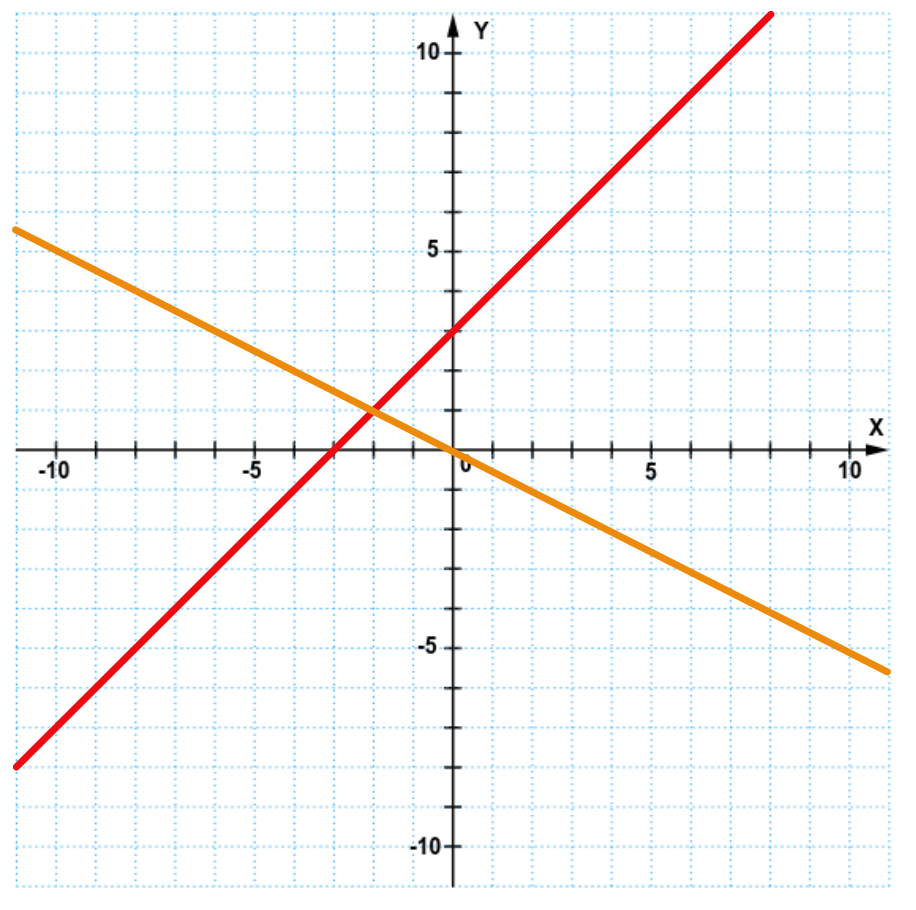
\includegraphics[scale=0.3]{sprv1_1.png}
		\end{center}
		Układ ten da się zapisać w postaci:}
	{\UkladRownan{y=-x+3}{y=-\frac{1}{2}x}}
	{\UkladRownan{y=x+3}{y=-\frac{1}{2}x}}
	{\UkladRownan{y=-x-3}{y=\frac{1}{2}x}}
	{\UkladRownan{y=x-3}{y=\frac{1}{2}x}}
	

	
	\Zadanie{Zapisać równanie okręgu o środku $S=(-4,2)$ i promieniu 4.}{\vspace{0.5cm}	\begin{center}
			.................................................................................................
	\end{center}}
	
	\begin{center}
		
		\begin{tabular}{|c|c|c|c|c|c|c|c|c|c|}\hline
			Zadanie&1&2&3&4&5&6&7&8&9\\\hline
			Max&2&1&3&3&2&4&2&1&2\\\hline
			Punkty&&&&&&&&&\\\hline
		\end{tabular}
	\end{center}
\end{document}

